\documentclass[tikz,border=5pt]{standalone}
\usepackage{fontspec}
\setmainfont{Times New Roman}
\usepackage{unicode-math}
\setmathfont{Cambria Math}
\usetikzlibrary{shapes.geometric,positioning,fit,backgrounds,arrows.meta,calc}

\begin{document}
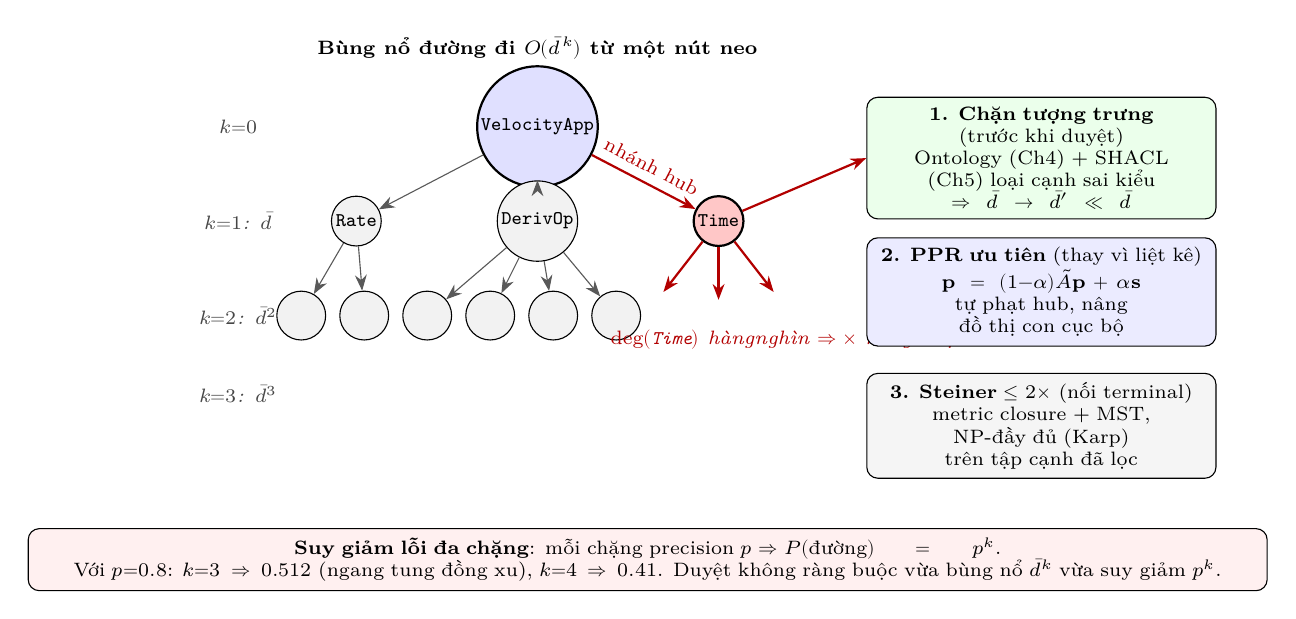
\begin{tikzpicture}[
  node/.style={circle, draw, minimum size=0.62cm, font=\scriptsize, inner sep=1pt},
  seed/.style={node, fill=blue!12, thick},
  hub/.style={node, fill=red!22, thick},
  leaf/.style={node, fill=gray!10},
  arrow/.style={-{Stealth[length=2mm]}, gray!70!black},
  cut/.style={-{Stealth[length=2mm]}, thick, red!70!black},
  label/.style={font=\scriptsize\itshape, text=gray!55!black},
  box/.style={draw, rounded corners, align=center, font=\scriptsize, text width=4.2cm},
]

% === Title ===
\node[font=\scriptsize\bfseries] at (3.2, 4.4) {Bùng nổ đường đi $O(\bar{d}^{\,k})$ từ một nút neo};

% === Layered tree: seed -> level1 -> level2 -> hub explosion ===
\node[seed] (s) at (3.2, 3.4) {\texttt{VelocityApp}};

\node[leaf] (a1) at (0.9, 2.2) {\texttt{Rate}};
\node[leaf] (a2) at (3.2, 2.2) {\texttt{DerivOp}};
\node[hub]  (a3) at (5.5, 2.2) {\texttt{Time}};

\node[leaf] (b1) at (0.2, 1.0) {};
\node[leaf] (b2) at (1.0, 1.0) {};
\node[leaf] (b3) at (1.8, 1.0) {};
\node[leaf] (b4) at (2.6, 1.0) {};
\node[leaf] (b5) at (3.4, 1.0) {};
\node[leaf] (b6) at (4.2, 1.0) {};

\draw[arrow] (s) -- (a1);
\draw[arrow] (s) -- (a2);
\draw[cut]   (s) -- (a3) node[midway, above, font=\scriptsize, text=red!70!black, sloped] {nhánh hub};

\foreach \from/\to in {a1/b1,a1/b2,a2/b3,a2/b4,a2/b5,a2/b6}
  \draw[arrow] (\from) -- (\to);

% hub fan-out (many edges)
\draw[cut] (a3) -- ++(0.7,-0.9);
\draw[cut] (a3) -- ++(0.0,-1.0);
\draw[cut] (a3) -- ++(-0.7,-0.9);
\node[label, text=red!70!black] at (6.4, 0.7) {$\deg(\texttt{Time})$ hàng\\ nghìn $\Rightarrow\times$ hàng triệu};

% === Depth annotations ===
\node[label] at (-0.6, 3.4) {$k{=}0$};
\node[label] at (-0.6, 2.2) {$k{=}1$: $\bar{d}$};
\node[label] at (-0.6, 1.0) {$k{=}2$: $\bar{d}^2$};
\node[label] at (-0.6, 0.0) {$k{=}3$: $\bar{d}^3$};

% === Bounding strategies (right column) ===
\node[box, fill=green!8] (prune) at (9.6, 3.0)
  {\textbf{1. Chặn tượng trưng} (trước khi duyệt)\\
   Ontology (Ch4) + SHACL (Ch5) loại cạnh sai kiểu\\
   $\Rightarrow \bar{d}\to\bar{d}'\ll\bar{d}$};

\node[box, fill=blue!8] (ppr) at (9.6, 1.3)
  {\textbf{2. PPR ưu tiên} (thay vì liệt kê)\\
   $\mathbf{p}=(1{-}\alpha)\tilde{A}\mathbf{p}+\alpha\mathbf{s}$\\
   tự phạt hub, nâng đồ thị con cục bộ};

\node[box, fill=gray!8] (steiner) at (9.6, -0.4)
  {\textbf{3. Steiner $\le 2\times$} (nối terminal)\\
   metric closure + MST, NP-đầy đủ (Karp)\\
   trên tập cạnh đã lọc};

\draw[cut] (a3) -- (prune.west);

% === Error cascade footnote ===
\node[box, fill=red!6, text width=15.5cm] (err) at (4.6, -2.1)
  {\textbf{Suy giảm lỗi đa chặng}: mỗi chặng precision $p$ $\Rightarrow$ $P(\text{đường})=p^{k}$.\\
   Với $p{=}0.8$: $k{=}3\Rightarrow0.512$ (ngang tung đồng xu), $k{=}4\Rightarrow0.41$. Duyệt không ràng buộc vừa bùng nổ $\bar{d}^k$ vừa suy giảm $p^k$.};

\end{tikzpicture}
\end{document}
